\documentclass[12pt]{article}
\usepackage[hmargin=1in,vmargin=1in]{geometry}
\usepackage{amsmath}
\usepackage{amssymb}
\usepackage{amsthm}
\usepackage{setspace}
\usepackage{graphicx}
\usepackage{sectsty}
\usepackage{fancyvrb}
\usepackage{mathtools}
\usepackage{float}
\usepackage[caption = false]{subfig}
\usepackage{verbatim}
\usepackage[flushleft]{threeparttable}
\usepackage[usenames, dvipsnames]{color}

\definecolor{cuse}{RGB}{212, 69, 0}
\definecolor{uva}{RGB}{0, 55, 119}

% Make all of the environments for different proof elements
\newtheorem{theorem}{Theorem}[section]
\newtheorem{lemma}[theorem]{Lemma}
\newtheorem{proposition}[theorem]{Proposition}
\newtheorem{corollary}[theorem]{Corollary}

\sectionfont{\large}
\subsectionfont{\normalsize}

\begin{document}

% Begin by using non-standard footnotes
\renewcommand*{\thefootnote}{\fnsymbol{footnote}}

% Basic title page for the document

\begin{titlepage}
\begin{doublespacing}
    \begin{center}
        \vspace*{1cm}
        \Large
        \textbf{Wisdom of the Crowds:}
        
        \vspace{0.5cm}
        Modeling Real-Time Win Probabilities With Twitter\\
        \large
        \vspace{1cm}
        David Freed and Samuel Green\\ \vspace{0cm}
        Applied Mathematics 221 \\
        April 30, 2016 \\
       \end{center}
       
       \vspace{3cm}
       
       % Abstract
	\begin{center}
	    \textbf{Abstract} \\
	    Past research has considered the ... We ... 
	\end{center}

\end{doublespacing}
\end{titlepage}

% Change back to use Arabic footnotes
\renewcommand*{\thefootnote}{\arabic{footnote}}

\setcounter{page}{1}
\newpage

\tableofcontents
\newpage
\begin{doublespacing}

% Introduction
\section{Introduction}

The wisdom of the crowds is not a new phenomenon. Economists treat the collective opinion of independent rational agents as sacrosanct; efficient market hypotheses are, at their core, expressing a fundamental belief in the wisdom of the crowds. Statisticians can explain the idea as the reduction of systemic risk---the variance of the sum of $n$ independent and identically distributed random variables is smaller than the variance of any individual r.v. by a factor of $\frac{1}{n}$. In politics, prediction markets have quickly become a better predictor of election results than polls or the opinions of the experts\footnote{http://www.wnd.com/2016/01/prediction-markets-more-accurate-than-polls}.

The last example evidences the importance of being able to properly assess the wisdom of the crowds. While betting on political elections is illegal in the United States, the number of bets on the current presidential race is up fourfold since 2012 in Ireland.\footnote{http://abcnews.go.com/Politics/las-vegas-bets-hillary-clinton-literally/story?id=30897911} Betfair, the largest online betting exchange for U.S. presidential elections, has nearly one million users and records nearly seven million transactions a day, which it claims is ``more than all European stock exchanges combined''.\footnote{http://corporate.betfair.com/about-us/betfair-facts.aspx} In this cutthroat industry, any edge a gambler can get matters. 

The betting market on politics pales next to the worldwide sports betting market---a colossal enterprise whose size experts ballpark at around \$1 trillion dollars a year. In a market with roughly the GDP of Indonesia, understanding the underlying statistics (in this case, the relative quality of the teams) is fundamental. Any bettor who can consistently outperform the crowds can turn a predictable profit; one has to win only 52.4 percent of his bets to break even in Vegas. 

In our paper, we tackle the common questions about the wisdom of the crowds from a different angle: instead of asking whether crowds or experts, alone or in aggregate, can predict games before they happen, we look at their ability to understand and predict games that are ongoing. We consider Twitter data from 43 games in the National Collegiate Athletic Association (henceforth, ``NCAA'') Men's Basketball Tournament (henceforth, ``March Madness'') to identify metrics that gauge the level of interest and the sentiment of the crowd at any point in time. 

The justification for using Twitter as a predictive mechanism is simple: it can update far quicker than standard predictors like the margin of the game. If a star player goes down with injury or picks up a fourth or fifth foul---forcing him out of the game---the immediate effect will not be seen in the margin, but Twitter users will be able to accurately process the effect it will have on the game. Likewise, while Twitter can distinguish margins that are unsustainable (e.g. leads built on fluky plays or low-percentage shots) and those that are not, standard statistical models have a difficult time doing so. 

Prior research has taken a cursory look at these questions; previous studies of National Football League (henceforth, ``NFL'') games identified that the volume of Tweets before a game is predictive of the final outcome and that Twitter is reactive to big plays in the game. Our work builds upon these analyses, not only by substantiating prior results for a different sport\footnote{Given the differences between football and basketball, this is a non-trivial contribution. Since basketball has far fewer breaks than football, one might imagine that Twitter would be significantly slower to reach to big events (fewer timeouts and breaks of play with which to process what happened). We show this not to be true in the Empirical Results section.} but also by distinguishing between Tweet volume and Tweet sentiment. Prior papers considered only the volume of Tweet in each contest to measure the wisdom of the crowd; we use a sentiment classifier to determine how Twitter feels about both teams and how that evolves over the course of the game. In our Empirical Results section, we demonstrate that Twitter sentiment has predictive power that Twitter volume does not.  

Our paper has three main results. First, to establish a baseline for our future analysis, we demonstrate empirically that Twitter is responsive to important game events---Twitter volume and sentiment will increase in response to salient changes in the score. This provides evidence for our initial claim that Twitter is responsive to the events currently going on in the game.  

After showing that Twitter can capture what has happened in the past, we argue that Twitter is a useful predictor of what happens in the future. Our second result demonstrates that Twitter sentiment and Twitter volume is a statistically significant predictor of future changes in margin; the aggregate Twitter sentiment in any period\footnote{This is roughly measured as the support for one team minus the support for another team.} is predictive of the change in margin in the next period. Here we find evidence for our prior claim about unobservable data---while margins tend to show mean reversion (i.e. teams that are up by a lot in period $t$ tend to see their margin shrink in period $t+1$) as a whole, Twitter sentiment helps to distinguish which leads will continue to increase. 

Our final result tests whether Twitter data can be used as an effective predictor of the final result at any point during the game. We use logistic regression models to incorporate the sentiment in a given period. We find that the Twitter sentiment is only statistically significant for about the final quarter of the game, but models that include Twitter sentiment outperform standard models\footnote{For the purposes of our analysis, we cite the logistic prediction models rolled out by FiveThirtyEight during this year's March Madness as the standard model for predicting the end of the game} at every single minute of the game. We conclude by showing that incorporating Twitter sentiment is more valuable than simply incorporating raw Twitter volume, as other papers have done. 

The remainder of the paper proceeds as follows. In Section 2, we review the brief literature on the subject, demonstrating both the advances and the gaps in prior research. In Section 3, we detail our data collection process, explaining how we matched gametime data (e.g. ``7:30 remaining in first half'') to real-time data (e.g. ``9:30 PM'') and discussing the construction of both our relevance and sentiment classifiers. In Section 4, we provide an overview of our empirical results and a thorough discussion of the aforementioned three main results and their significance. In Section 5, we conclude and discuss the important caveats and extensions to our work. 

% Literature Review
\section{Overview of Related Literature}

Previous literature has established taht useful modeling information can be
derived from Twitter data, some including work using sentiment analysis, with the body of work mostly focused on the NFL. 

A real-time system was built in 2012 using volumes of 
tweets related to National Football League (NFL) games to 
isolate significant game
events=. That project characterized a 
difference between human- and machine-generated tweets
based on posting rates, and, by discriminating between 
different varieties of users, the system could 
identify events in near real-time. The event detection
system leveraged pre-selected sets of hashtags
to isolate relevant tweets as input to the system. (Zhao et al, 
2012)\footnote{http://arxiv.org/pdf/1205.3212v1.pdf}. 

Sentiment analysis has also been previously applied
to Twitter data to a predictive model for NFL games. 
In 2013, Sinha et al. found that Twitter data collected
in advance of weekly NFL games could be used effectively
to predict the outcomes of games more successfully than
methods using other traditional statistical models. Their
work used a dataset of tweets collected over periods 
in advance of games and also collected tweets by 
building sets of hashtags related to participant teams (Sinha et al., 2013).\footnote{https://www.cs.cmu.edu/~nasmith/papers/sinha+dyer+gimpel+smith.mlsa13.pdf}

% Literature Review
\section{Data Overview}

Our dataset consists of approximately 1 million Tweets made during the 2016 National Collegiate Athletic Association (henceforth, ``NCAA") Men's Basketball Tournament (henceforth, ``March Madness''). Before describing how we acquired and classified Tweets, we briefly describe March Madness and the basketball-related data we collected. 

\subsection{Game Data}

March Madness, the largest single-elimination tournament in major American sports, is one of the most important events on the U.S. sporting calendar. The tournament takes place from mid-March to early April, with the 68-team field shrinking to sixteen after the first weekend. On the following weekend, the so-called ``Sweet Sixteen" compete for a spot in the ``Final Four"---the given name for the national semifinals. The 67-game tournament, which takes teams from across the country,\footnote{In fact, nearly every major school is eligible to compete in March Madness. The tournament reserves 33 spots for the winners of each major Division I athletic conference, leaving an automatic berth available for 351 colleges and universities across the nation} is the NCAA's primary source of revenue---in 2015, it comprised 90 percent of the organization's total revenue. 

We chose to look at March Madness game data because of the level of excitement surrounding the event. Unlike other sports that share the same athletic calendar---most prominently, the National Basketball Association (henceforth, ``NBA'')---there are rarely more than two March Madness games occurring at once and so the entire focus is on the current game. 

The level of interest surrounding an average March Madness game is much higher than that for a regular season mid-week NBA contest; the tournament encourages fans, regardless of their level of expertise, to fill out a bracket predicting the outcome. This cultural phenomenon has exploded in recent years, with ESPN receiving 13 million brackets this year. From the brackets arises an intense gambling market (more than \$9 billion in 2016), raising interest and attention in the games. 

%% Image 1: Basic Result From Box Score Scraper
\begin{figure} [H]
	\centering
	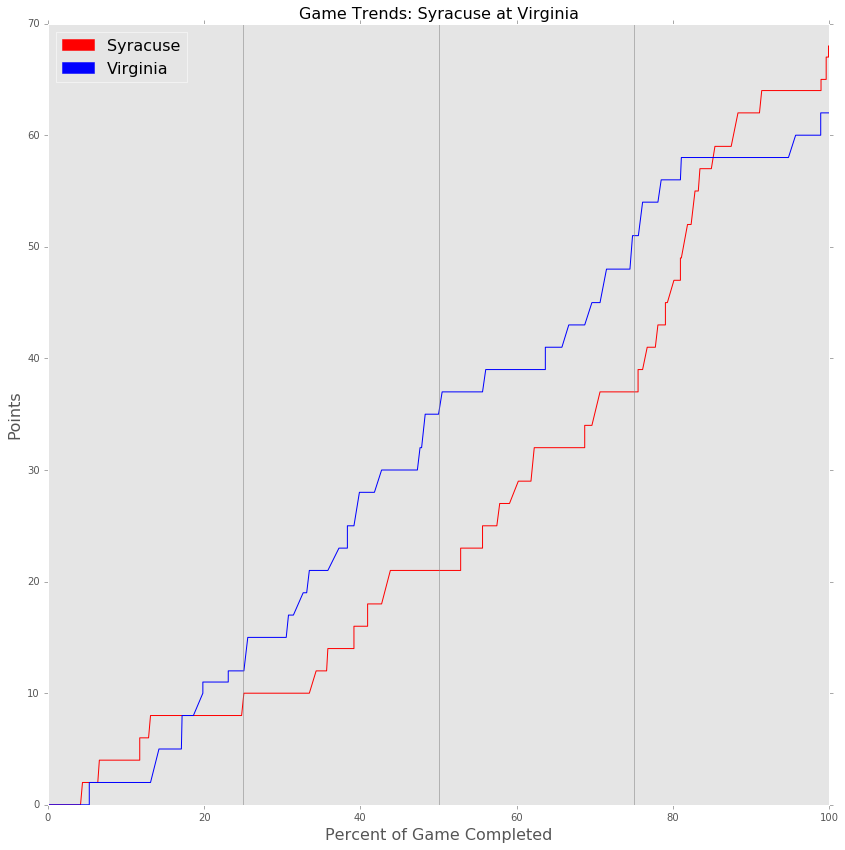
\includegraphics[scale = 0.4] {Images/Cuse_UVA_MarginOverTime.png} 
	\caption{Score over time for Syracuse-Virginia Elite Eight contest}
\end{figure}

For each 2016 March Madness contest, we scraped \texttt{ESPN.com} to secure play-by-play data for each contest. From the website, we were able to get the scores for each team at every point in time, as well as a description of every event (i.e. ``Paige, Marcus hits a three-pointer"). Figure 1 above shows the evolution of a Syracuse-Virginia Elite Eight contest, with Syracuse coming back from a 14-point deficit to take a late lead and storm into the Final Four. 

\subsection{Twitter Data}

After obtaining our game data, we sought to collect a series of Tweets for each event to gauge public sentiment while the game was happening. In order to do this, we set up a Tweet listener while the game was actually going on, recording the Tweets as they were sent for an hour before and an hour after each game. 

In order to detect which Tweets were relevant, we only pulled Tweets that had a certain set of hashtags. Following the blueprint of Sinha et al. (2013), we constructed a set of Tweets associated with each game manually, scrolling through the official Twitter accounts of each individual team and adding the most commonly used hashtags to our list. 
\vspace{1cm}
%% Image 2: Basic Example Set of Hashtags
\begin{figure} [H]
    \begin{center}
    \#\texttt{NCAATournament} \#\texttt{MarchMadness} \#\texttt{LetsDance} \\ 
    \#\texttt{NCAATOURNAMENT} \#\texttt{CBB} \#\texttt{NCAAB} \\ 
    \#\texttt{SyracusevsVirginia} \textcolor{cuse}{\#\texttt{Syracuse}} \textcolor{cuse}{\#\texttt{Cuse}} \\ 
    \textcolor{cuse}{\#\texttt{OrangeCrush}} \textcolor{cuse}{\#\texttt{CuseMode}} \textcolor{uva}{\#\texttt{Virginia}} \\ 
    \textcolor{uva}{\#\texttt{UVA}} \textcolor{uva}{\#\texttt{GoHoos}} \textcolor{uva}{\#\texttt{Cavaliers}} \\
    \caption{Set of NBA hashtags for UVA-Syracuse Elite Eight game.}
    \end{center}
\end{figure}

Figure 2 above demonstrates the set of hashtags used for the UVA-Syracuse game. Hashtags in black are hashtags that were not related to either team and common to all sets of tags.\footnote{With the caveat that the final Tweet, "\#SyracusevsVirginia", was altered in each case to refer only to the teams playing in the game.} The other hashtags were taken directly from the official Twitter accounts of the two schools and are colored in relation to which school they refer to. 

To get a sufficient cross-section of data, we took Tweets corresponding to 43 separate games. Fifty-four of the 68 teams participated in at least one game in our dataset. All in all, we collected over 1 million Tweets, with an average of roughly 21,000 Tweets per game. 

%% Image 3: Number of Tweets as a Histogram
\begin{figure} [H]
	\centering
	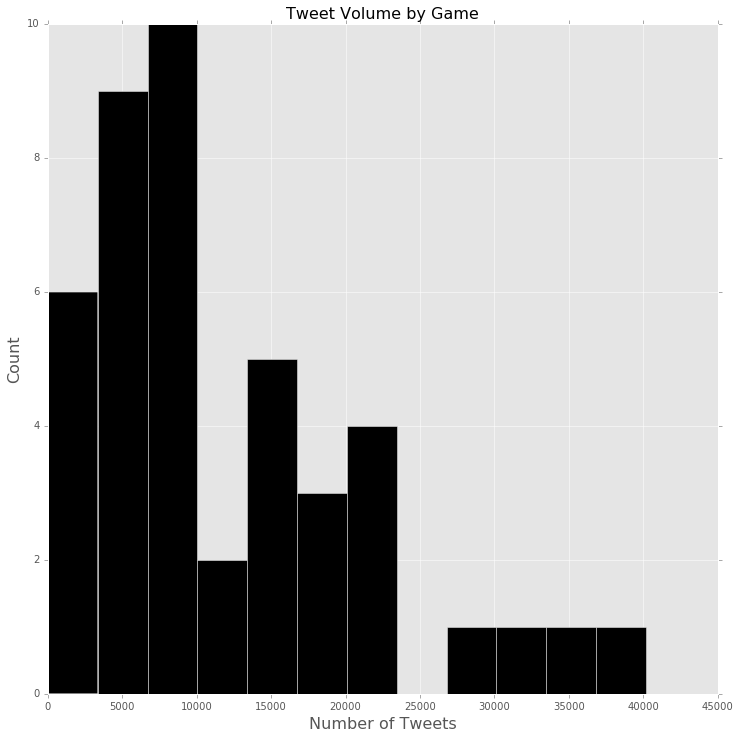
\includegraphics[scale = 0.4] {Images/TweetVolumeByGame.png} 
	\caption{Tweet volume by contest}
\end{figure}

Figure 3 above shows the distribution of Tweets per game. The number of Tweets increased as the tournament went on; while first-round games had an average of just about 12.7 thousand Tweets a contest, there were an average of 15.8 thousand Tweets about each Sweet Sixteen contest in our dataset. Figure 3 excludes the national title game between Villanova and the University of North Carolina, which garnered just under 160,000 total tweets---by far the most in the dataset. 

Once we had the two datasets, we set out to match the two to one another. Our source for game data did not log the exact moment at which each event occurred in real time, just in game time. To map game time (i.e. ``11:30, first half'') to real time (``9:30 PM''), we used a rough approximation algorithm. For each game, we manually took the beginning and end times of each game from \texttt{ESPN.com} and \texttt{@marchmadness}, the official Twitter handle of the NCAA Tournament and used that information to estimate the length of each half. From that data, we estimated the time each event happened as a function of the length of each half and the time remaining in each half, using a modified uniform approximation to match game times to real times. 

%% Image 4: Twitter Volume over time 
\begin{figure} [H]
	\centering
	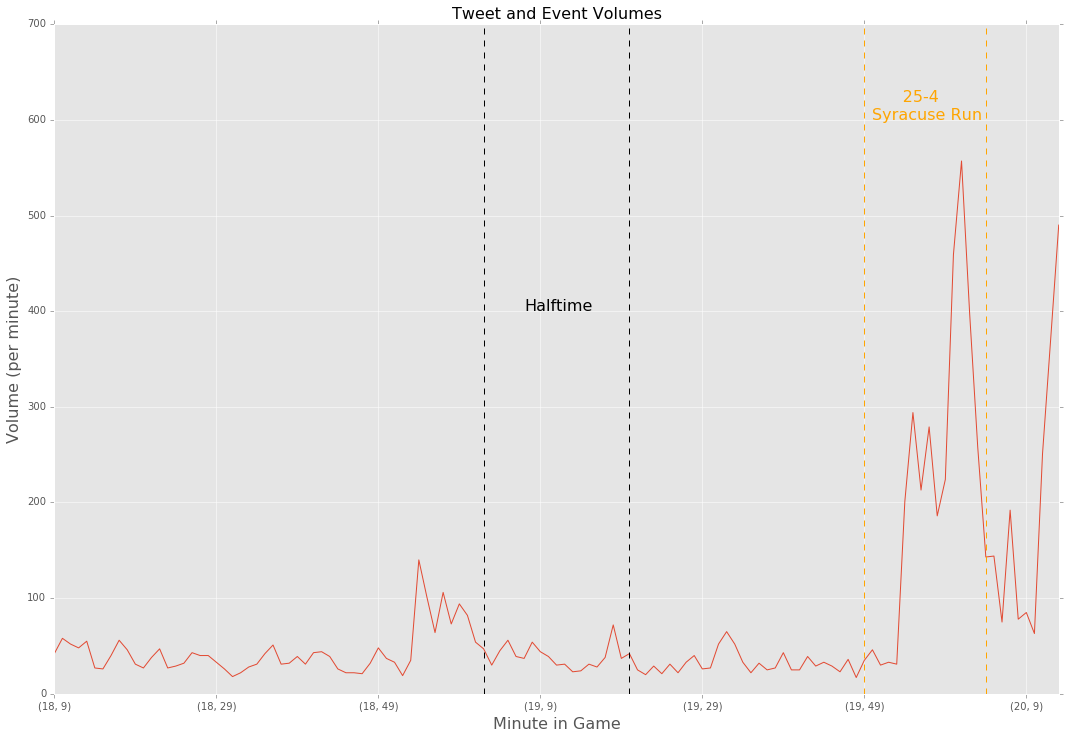
\includegraphics[scale = 0.4] {Images/Total_TweetVolume.png} 
	\caption{Tweet counts over time for UVA-Syracuse}
\end{figure}

Figure 4 above demonstrates the results of the mapping, which allowed us to identify exactly when halftime and key game events occurred in real time. As seen in the above graph, there was a significant spike in Twitter traffic during the pivotal moments of the game---a 25-4 run by Syracuse that brought the team from 14 points down into the lead. The associated large spike in Twitter traffic seen in the above figure reflects a common trend across the data: when the game got more exciting, Tweet volume spiked. 

The next classification we made to the data was to classify each Tweet according to which team it related to. Since the eventual goal of the project was to be able to classify public sentiment towards any given team at any point in time, our intermediate step was to associate each Tweet with a team based on the content of its message. 

To classify the subject of each Tweet, we created a list of relevant tags\footnote{In addition to using the tags shown in Figure 2, we scraped the last names of the seven best players for each team and the coach of the team. In many cases, we found that Tweets included both team names (i.e. `` ... \#Virginia \#Syracuse'') but were actually about one team or the other. Including the last names of the players increased the accuracy of our classifier, since it better differentiated amongst these Tweets.} for each time and identified how often they showed up in the Tweet. From this, we computed a weighted relevance score for both teams, dividing the Tweets according to their relevance score for each team (i.e. those with a higher relevance score for Syracuse were tagged as `Syracuse-related' Tweets).  

%% Image 5: Twitter Volume over time by subject
\begin{figure} [H]
	\centering
	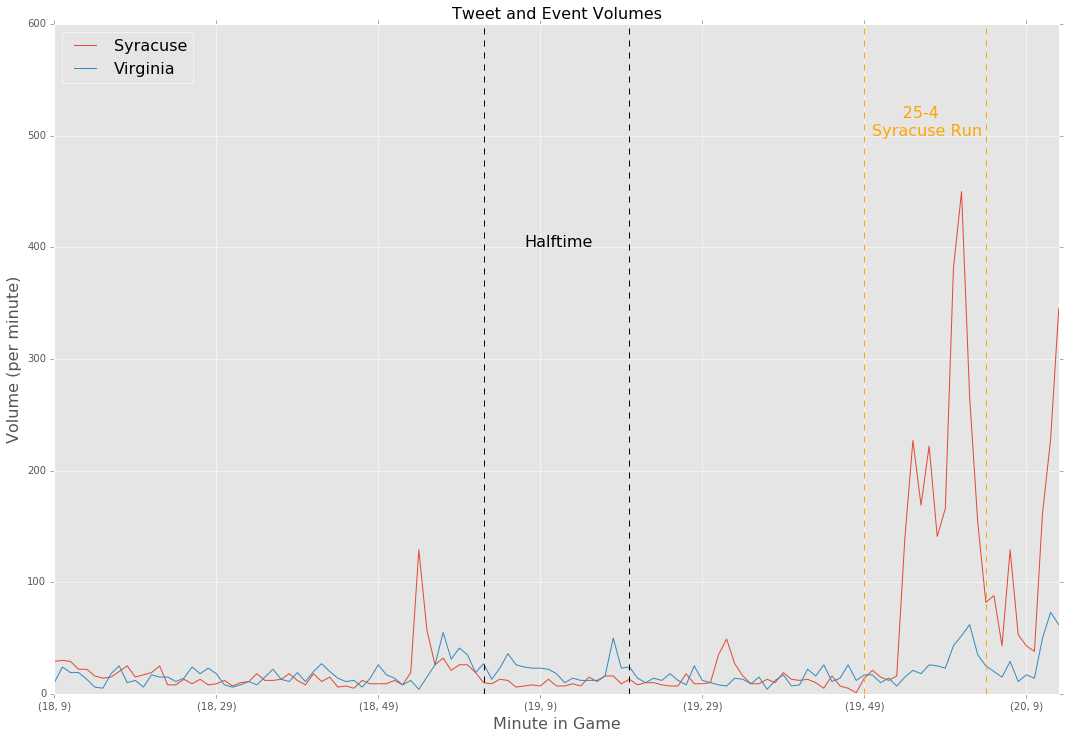
\includegraphics[scale = 0.4] {Images/Cuse_UVA_TweetVolume.png} 
	\caption{Tweets counts by subject over time for UVA-Syracuse}
\end{figure}

Figure 5 above breaks down the Tweet volume data by team, demonstrating that the spike in traffic during Syracuse' run comes almost entirely from people Tweeting about their comeback. We can see that when trailing early in the game, very few people were Tweeting about Syracuse; likewise, when Virginia opened up at a 14-point lead at halftime, they saw a brief bump in traffic during the 20-minute intermission. 

The final step in our data collection was to classify the sentiment of each Tweet. In order to tell whether public opinion was positive or negative for each team over time, we constructed a sentiment classifier for individual Tweets. We chose a linear-kernel Support Vector Machine as our primary classifier, using a standard bag-of-words methodology and training the model on a prior labeled corpus of over 4000 words\footnote{We had to make minor mechanical adjustments to the model due to the oddities of the language surrounding basketball; while words like `dirty', `filthy', and `disgusting' would be classified as negative sentiments in almost any social context, they are the highest of compliments that can be paid on a basketball court}. 

%% Image 6: Twitter sentiment over time by team
\begin{figure} [H]
	\centering
	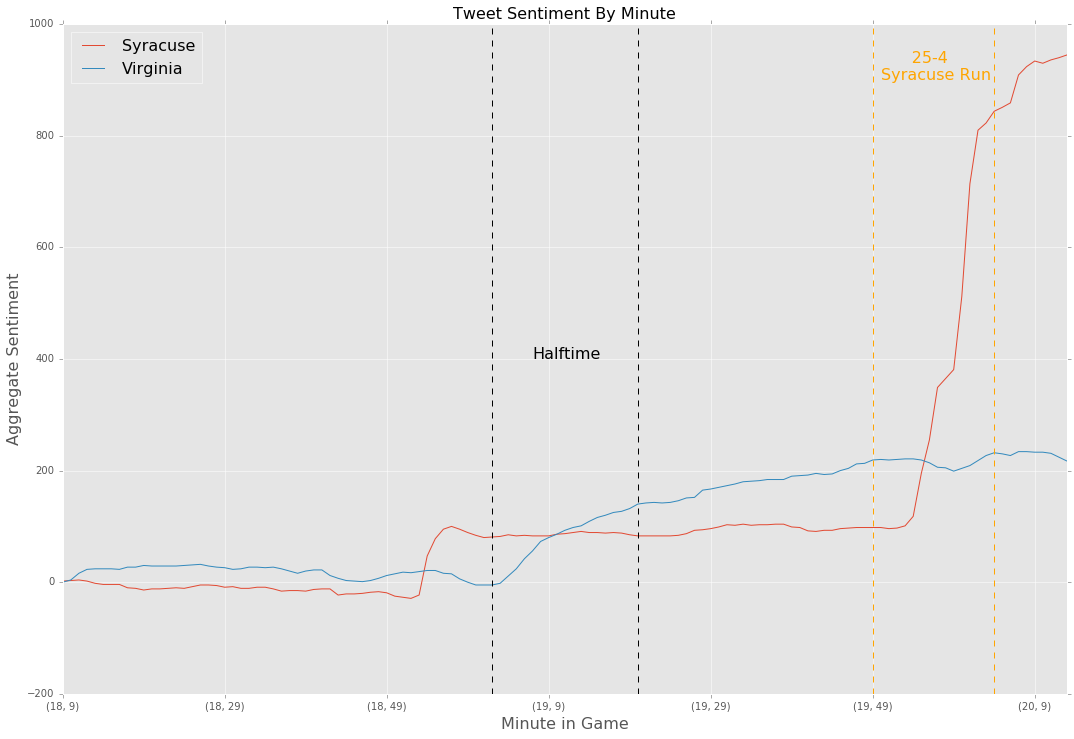
\includegraphics[scale = 0.4] {Images/Cuse_UVA_TweetSentiment.png} 
	\caption{Tweet sentiment over time for UVA-Syracuse}
\end{figure}

Figure 6 above demonstrates the results of our classifier. We grouped Tweets into three categories: positive, negative, and neutral. In order to come up with an aggregate sentiment at any point in time, we took a simple linear combination of the three numbers---with our weights determined by the relative sensitivity of our classifier.\footnote{Since our classifier was more sensitive to positive speech than negative speech, we gave a higher coefficient to the amount of negative Tweets, assuming that they were an under-representation of the general sentiment}. 

The results, demonstrated above, were fascinating. During the Syracuse-UVA game, we can clearly see that as Syracuse falls behind, public sentiment drops into the negatives. An 8-0 run during the latter stages of the first half generates a lot of positive public sentiment, but during the half, the public begins to support Virginia (who has a 14-point lead). As Syracuse makes its comeback in the second half, however, Virginia plateaus and sentiment on Twitter shifts very strongly towards the Orange. As demonstrated in the forthcoming sections, this is evidence of the reactionary public sentiment to changes in the box score. 

% Literature Review
\section{Empirical Results}

% Literature Review
\section{Discussion}

% Literature Review
\section{Tables and Figures}

%% Table 1: How Twitter Responds to Changes in Margin (Sentiment)
\begin{table}[H] 
\centering 
\caption{Twitter Responsiveness to Game Events (pt. 1)} 
\label{} 
\begin{tabular*}{\textwidth}{@{\extracolsep{\fill}}lccc} 
\hline 
\hline
 & \multicolumn{3}{c}{\textit{Dependent variable:}} \\ 
\cline{2-4} 
\\[-3.0ex] & \multicolumn{3}{c}{SentDiff\_Period} \\ 
\\[-1.5ex] & (1) & (2) & (3)\\ 
\hline
 Margin\_Period\_Lag1 & 0.891$^{**}$ & 0.881$^{**}$ & 0.910$^{**}$ \\ 
  & (0.367) & (0.366) & (0.370) \\ 
 Margin\_Period\_Lag2 &  &  & 0.864$^{**}$ \\ 
  &  &  & (0.377) \\ 
 Vegas\_Line &  & $-$1.008$^{***}$ & $-$0.973$^{***}$ \\ 
  &  & (0.231) & (0.237) \\ 
 QualityDiff &  & 35.390$^{***}$ & 32.811$^{***}$ \\ 
  &  & (10.041) & (10.304) \\ 
 TwitterDiff &  & $-$0.004 & $-$0.006 \\ 
  &  & (0.011) & (0.011) \\ 
 Min\_End &  & 0.068 & 0.061 \\ 
  &  & (0.075) & (0.079) \\ 
\hline \\[-1.8ex] 
Observations & 1,306 & 1,306 & 1,266 \\ 
R$^{2}$ & 0.005 & 0.021 & 0.023 \\ 
Adjusted R$^{2}$ & 0.004 & 0.017 & 0.018 \\ 
Residual Std. Error & 30.443 & 30.238 & 30.562 \\ 
F Statistic & 5.897$^{**}$ & 5.548$^{***}$ & 4.972$^{***}$ \\ 
\hline 
\hline \\[-1.8ex] 
\end{tabular*} 
\end{table} 

%% Table 2: How Twitter Responds to Changes in Margin (Volume)
\begin{table}[H] 
\centering 
\caption{Twitter Responsiveness to Game Events (pt. 2)} 
\label{} 
\begin{tabular*}{\textwidth}{@{\extracolsep{\fill}}lccc} 
\hline 
\hline
 & \multicolumn{3}{c}{\textit{Dependent variable:}} \\ 
\cline{2-4} 
\\[-3.0ex] & \multicolumn{3}{c}{VolDiff\_Period} \\ 
\\[-1.5ex] & (1) & (2) & (3)\\ 
\hline
 Margin\_Period\_Lag1 & 6.253$^{***}$ & 5.877$^{***}$ & 6.028$^{***}$ \\ 
  & (1.259) & (1.237) & (1.246) \\ 
 Margin\_Period\_Lag2 &  &  & 4.779$^{***}$ \\ 
  &  &  & (1.268) \\ 
 Vegas\_Line &  & $-$1.454$^{*}$ & $-$1.416$^{*}$ \\ 
  &  & (0.781) & (0.797) \\ 
 QualityDiff &  & 129.964$^{***}$ & 122.143$^{***}$ \\ 
  &  & (33.914) & (34.662) \\ 
 TwitterDiff &  & 0.165$^{***}$ & 0.168$^{***}$ \\ 
  &  & (0.036) & (0.037) \\ 
 Min\_End &  & $-$0.630$^{**}$ & $-$0.679$^{**}$ \\ 
  &  & (0.253) & (0.267) \\ 
\hline \\[-1.8ex] 
Observations & 1,306 & 1,306 & 1,266 \\ 
R$^{2}$ & 0.019 & 0.063 & 0.073 \\ 
Adjusted R$^{2}$ & 0.018 & 0.060 & 0.069 \\ 
Residual Std. Error & 104.377 & 102.132 & 102.812 \\ 
F Statistic & 24.685$^{***}$  & 17.550$^{***}$ & 16.599$^{***}$ \\
\hline 
\hline \\[-1.8ex] 
\end{tabular*} 
\end{table} 

%% Table 3: Twitter Sensitivity to Game Events During Closing Minutes
\begin{table}[H] 
\centering 
\caption{Twitter Responsiveness to Game Events (Closing Minutes)} 
\label{} 
\begin{tabular*}{\textwidth}{@{\extracolsep{\fill}}lcccc} 
\hline 
\hline
 & \multicolumn{4}{c}{\textit{Dependent variable:}} \\ 
\cline{2-5} 
\\[-3.0ex] & \multicolumn{2}{c}{SentDiff\_Period} & \multicolumn{2}{c}{VolDiff\_Period} \\ 
\\[-1.5ex] & (1) & (2) & (3) & (4)\\ 
\hline
 Margin\_Period & 3.080$^{***}$ &  & 9.598$^{***}$ &  \\ 
  & (0.898) &  & (2.980) &  \\ 
 Margin\_Period\_Lag1 &  & 1.325 &  & 7.570$^{**}$ \\ 
  &  & (0.934) &  & (3.071) \\ 
 Vegas\_Line & $-$1.691$^{***}$ & $-$1.802$^{***}$ & 1.061 & 0.671 \\ 
  & (0.585) & (0.594) & (1.941) & (1.953) \\ 
 QualityDiff & 54.306$^{**}$ & 61.013$^{**}$ & 44.282 & 60.681 \\ 
  & (25.706) & (26.013) & (85.282) & (85.559) \\ 
 TwitterDiff & $-$0.012 & $-$0.012 & 0.451$^{***}$ & 0.447$^{***}$ \\ 
  & (0.028) & (0.028) & (0.092) & (0.092) \\ 
 Min\_End & $-$0.526 & $-$0.719 & $-$2.755 & $-$3.466 \\ 
  & (0.740) & (0.751) & (2.455) & (2.470) \\ 
\hline \\[-1.8ex] 
Observations & 316 & 316 & 316 & 316 \\ 
R$^{2}$ & 0.068 & 0.039 & 0.133 & 0.121 \\ 
Adjusted R$^{2}$ & 0.053 & 0.024 & 0.119 & 0.107 \\ 
Residual Std. Error & 37.840 & 38.427 & 125.537 & 126.387 \\ 
F Statistic & 4.535$^{***}$ & 2.520$^{**}$ & 9.490$^{***}$ & 8.531$^{***}$ \\ 
\hline 
\hline \\[-1.8ex] 
\end{tabular*} 
\end{table} 

%% Table 4: Can Twitter Sentiment Predict Future Margins
\begin{table}[H] 
\centering 
\caption{The Accuracy of the Crowds (pt. 1)} 
\label{} 
\begin{tabular*}{\textwidth}{@{\extracolsep{\fill}}lccc} 
\hline 
\hline
 & \multicolumn{3}{c}{\textit{Dependent variable:}} \\ 
\cline{2-4} 
\\[-3.0ex] & \multicolumn{3}{c}{Margin\_Period} \\ 
\\[-1.5ex] & (1) & (2) & (3)\\ 
\hline
 SentDiff\_Period\_Lag1 & 0.006$^{***}$ & 0.006$^{***}$ & 0.006$^{***}$ \\ 
  & (0.002) & (0.002) & (0.002) \\ 
 SentDiff\_Period\_Lag2 &  &  & 0.001 \\ 
  &  &  & (0.003) \\ 
 SentDiff\_Period\_Lag3 &  &  & $-$0.003 \\ 
  &  &  & (0.002) \\ 
 Vegas\_Line &  & 0.009 & 0.003 \\ 
  &  & (0.018) & (0.019) \\ 
 QualityDiff &  & 0.983 & 1.239 \\ 
  &  & (0.780) & (0.809) \\ 
 TwitterDiff &  & 0.0003 & 0.0002 \\ 
  &  & (0.001) & (0.001) \\ 
 Min\_End &  & 0.004 & 0.007 \\ 
  &  & (0.006) & (0.006) \\ 
\hline \\[-1.8ex] 
Observations & 1,306 & 1,306 & 1,226 \\ 
R$^{2}$ & 0.006 & 0.012 & 0.015 \\ 
Adjusted R$^{2}$ & 0.005 & 0.008 & 0.009 \\ 
Residual Std. Error & 2.342 & 2.338 & 2.344 \\ 
F Statistic & 7.250$^{***}$ & 3.106$^{***}$ & 2.638$^{**}$ \\ 
\hline 
\hline \\[-1.8ex] 
\end{tabular*} 
\end{table} 

%% Table 5:
\begin{table}[H] 
\centering 
\caption{The Accuracy of the Crowds (pt. 2)} 
\label{} 
\begin{tabular*}{\textwidth}{@{\extracolsep{\fill}}lcccc} 
\hline 
\hline
 & \multicolumn{4}{c}{\textit{Dependent variable:}} \\ 
\cline{2-5} 
\\[-3.0ex] & \multicolumn{4}{c}{Margin\_Period} \\ 
\\[-1.5ex] & (1) & (2) & (3) & (4)\\ 
\hline
  VolDiff\_Period\_Lag1 & 0.002$^{***}$ & 0.002$^{***}$ & 0.002$^{**}$ & 0.003$^{***}$ \\ 
  & (0.001) & (0.001) & (0.001) & (0.001) \\ 
 SentDiff\_Period\_Lag1 &  &  & 0.004 &  \\ 
  &  &  & (0.002) &  \\ 
 VolDiff\_Period\_Lag2 &  &  &  & 0.0004 \\ 
  &  &  &  & (0.001) \\ 
 VolDiff\_Period\_Lag3 &  &  &  & $-$0.002$^{**}$ \\ 
  &  &  &  & (0.001) \\ 
 Vegas\_Line &  & 0.006 & 0.009 & 0.0004 \\ 
  &  & (0.018) & (0.018) & (0.018) \\ 
 QualityDiff &  & 0.902 & 0.837 & 1.224 \\ 
  &  & (0.780) & (0.781) & (0.806) \\ 
 TwitterDiff &  & $-$0.00003 & 0.0001 & 0.00005 \\ 
  &  & (0.001) & (0.001) & (0.001) \\ 
 Min\_End &  & 0.005 & 0.005 & 0.008 \\ 
  &  & (0.006) & (0.006) & (0.006) \\ 
\hline \\[-1.8ex] 
Observations & 1,306 & 1,306 & 1,306 & 1,226 \\ 
R$^{2}$ & 0.009 & 0.014 & 0.016 & 0.021 \\ 
Adjusted R$^{2}$ & 0.008 & 0.010 & 0.011 & 0.015 \\ 
Residual Std. Error & 2.338 & 2.335 & 2.334 & 2.337 \\ 
F Statistic & 11.852$^{***}$ & 3.686$^{***}$ & 3.435$^{***}$ & 3.675$^{***}$  \\ 
\hline 
\hline \\[-1.8ex] 
\end{tabular*} 
\end{table} 

%% Table 6: Reversion to the Mean
\begin{table}[H] 
\centering 
\caption{Reversion to the Mean} 
\label{} 
\begin{tabular*}{\textwidth}{@{\extracolsep{\fill}}lcccc} 
\hline 
\hline
 & \multicolumn{4}{c}{\textit{Dependent variable:}} \\ 
\cline{2-5} 
\\[-3.0ex] & \multicolumn{4}{c}{Margin\_Period} \\ 
\\[-1.5ex] & (1) & (2) & (3) & (4)\\ 
\hline
 Margin\_TOT\_Lag1 & $-$0.018$^{**}$ & $-$0.023$^{***}$ & $-$0.019$^{**}$ & $-$0.024$^{***}$ \\ 
  & (0.008) & (0.008) & (0.008) & (0.008) \\ 
 SentDiff\_Total\_Lag1 &  & 0.001$^{**}$ &  & 0.001$^{**}$ \\ 
  &  & (0.0004) &  & (0.0004) \\ 
 VolDiff\_Total\_Lag1 &  &  & 0.00004 & 0.00005 \\ 
  &  &  & (0.0001) & (0.0001) \\ 
 Vegas\_Line & 0.005 & 0.016 & 0.005 & 0.017 \\ 
  & (0.018) & (0.019) & (0.018) & (0.019) \\ 
 QualityDiff & 1.679$^{**}$ & 1.364$^{*}$ & 1.631$^{**}$ & 1.303 \\ 
  & (0.802) & (0.815) & (0.805) & (0.819) \\ 
 TwitterDiff & 0.0004 & 0.0005 & 0.0003 & 0.0003 \\ 
  & (0.001) & (0.001) & (0.001) & (0.001) \\ 
 Min\_End & 0.002 & 0.001 & 0.002 & 0.002 \\ 
  & (0.006) & (0.006) & (0.006) & (0.006) \\ 
\hline \\[-1.8ex] 
Observations & 1,306 & 1,306 & 1,306 & 1,306 \\ 
R$^{2}$ & 0.011 & 0.014 & 0.011 & 0.015 \\ 
Adjusted R$^{2}$ & 0.007 & 0.010 & 0.007 & 0.009 \\ 
Residual Std. Error & 2.339 & 2.336 & 2.340 & 2.337 \\ 
F Statistic & 2.865$^{**}$ & 3.111$^{***}$ & 2.454$^{**}$ & 2.744$^{***}$ \\ 
\hline 
\hline \\[-1.8ex] 
\end{tabular*} 
\end{table} 

%% Table 7: Generalized Linear Model
\begin{table}[H] 
\centering 
\caption{Generalized Linear Model} 
\label{} 
\begin{tabular*}{\textwidth}{@{\extracolsep{\fill}}lcccc} 
\hline 
\hline
 & \multicolumn{4}{c}{\textit{Dependent variable:}} \\ 
\cline{2-5} 
\\[-3.0ex] & \multicolumn{4}{c}{Winner} \\ 
\\[-1.5ex] & (1) & (2) & (3) & (4)\\ 
\hline
 Vegas\_Line & $-$0.041$^{***}$ & $-$0.034$^{**}$ & $-$0.044$^{***}$ & $-$0.038$^{***}$ \\ 
  & (0.014) & (0.014) & (0.014) & (0.014) \\ 
 Margin\_TOT & 0.173$^{***}$ & 0.166$^{***}$ & 0.168$^{***}$ & 0.160$^{***}$ \\ 
  & (0.012) & (0.012) & (0.012) & (0.012) \\ 
 SentDiff\_Total &  & 0.001$^{***}$ &  & 0.001$^{***}$ \\ 
  &  & (0.0005) &  & (0.001) \\ 
 VolDiff\_Total &  &  & 0.0002$^{**}$ & 0.0002$^{**}$ \\ 
  &  &  & (0.0001) & (0.0001) \\ 
 Constant & $-$1.067$^{***}$ & $-$1.043$^{***}$ & $-$1.074$^{***}$ & $-$1.056$^{***}$ \\ 
  & (0.109) & (0.112) & (0.112) & (0.114) \\ 
\hline \\[-1.8ex] 
Observations & 1,346 & 1,346 & 1,346 & 1,346 \\ 
Log Likelihood & $-$594.303 & $-$590.365 & $-$591.049 & $-$587.436 \\ 
Akaike Inf. Crit. & 1,194.606 & 1,188.730 & 1,190.097 & 1,184.873 \\
\hline 
\hline \\[-1.8ex] 
\end{tabular*} 
\end{table} 

% Literature Review
\section{Bibliography}

% Literature Review
\section{Appendices}

\end{doublespacing}

\end{document}